
\documentclass[10pt,aspectratio=169]{beamer}

%================================================
% Theme
%================================================
\usetheme[numbering=fraction,progressbar=frametitle]{metropolis}

%================================================
% Packages
%================================================
\usepackage{amsmath,amssymb}
\usepackage{booktabs}
\usepackage{tikz}
\usetikzlibrary{automata,positioning,arrows.meta,calc,trees}
\usepackage[useregional]{datetime2}
\usepackage{xcolor}
\usepackage{listings}

%================================================
% Metadata
%================================================
\newcommand{\LastCompiled}{\DTMnow}

\title{Theory of Computation}
\subtitle{Lecture 5: Nondeterminism and Nondeterministic Finite Automata}
\author{Sheikh Azizul Hakim\\Lecturer, Department of CSE, BUET}
\date{Last compiled: \LastCompiled}

%================================================
% Listings
%================================================
\lstdefinestyle{code}{
  basicstyle=\ttfamily\small,
  frame=single,
  backgroundcolor=\color{black!4},
  rulecolor=\color{black!20},
  showstringspaces=false,
  columns=fullflexible,
  keepspaces=true
}
\lstset{style=code}

%================================================
% Helpers
%================================================
\newcommand{\eps}{\varepsilon}
\newcommand{\powset}[1]{2^{#1}}
\newcommand{\lang}[1]{\mathsf{#1}}

\tikzset{
  every state/.style={minimum size=8mm},
  >=Stealth,
  shorten >=1pt,
}

%================================================
\begin{document}

%================================================
\maketitle

%================================================
\begin{frame}[standout]
Sometimes finding a solution is hard.

But verifying a guessed solution is easy.
\end{frame}

%================================================
\section{Lecture 5A: The Philosophy of Nondeterminism}

%------------------------------------------------
\begin{frame}{The Central Question}

In deterministic computation, every step is forced.

\[
(\text{current state},\text{input symbol})
\longrightarrow
\text{exactly one next state}
\]

\vspace{1em}

Today we ask:

\begin{center}
What if a machine could explore many possibilities?
\end{center}

\pause

This idea is called \textbf{nondeterminism}.

\end{frame}

%------------------------------------------------
\begin{frame}{Find versus Verify}

Many computational tasks have two versions.

\vspace{0.5em}

\begin{center}
\begin{tabular}{lll}
\toprule
\textbf{Problem} & \textbf{Find} & \textbf{Verify} \\
\midrule
Maze & Find a path & Check a given path \\
Sudoku & Solve puzzle & Check a completed board \\
Password & Discover password & Test a candidate password \\
SAT & Find assignment & Check a given assignment \\
Proof & Find proof & Check a written proof \\
\bottomrule
\end{tabular}
\end{center}

\vspace{0.7em}

\pause
The second task is often much easier.

\end{frame}

%------------------------------------------------
\begin{frame}{Example: Maze}

Task:

\begin{center}
Find a path from the entrance to the exit.
\end{center}

\vspace{1em}

This may require search.

\pause

\vspace{1em}

But if someone gives us a candidate path, we can quickly check:

\begin{itemize}
\item Does it start at the entrance?
\item Does every step follow a valid corridor?
\item Does it end at the exit?
\end{itemize}

\vspace{0.5em}

\pause
Finding and verifying are different kinds of computation.

\end{frame}

%------------------------------------------------
\begin{frame}{Example: Sudoku}

Finding a solution may be difficult.

\vspace{1em}

Verifying a completed board is straightforward:

\begin{itemize}
\item Check every row.
\item Check every column.
\item Check every block.
\end{itemize}

\vspace{1em}

\pause
This distinction will reappear later in complexity theory as a central theme.

\end{frame}

%------------------------------------------------
\begin{frame}{The Nondeterministic Dream}

Imagine a machine that can say:

\begin{quote}
Let me guess the correct branch of the search.
\end{quote}

\vspace{1em}

If the guess can be verified, the machine accepts.

\pause

\vspace{1em}

This is not how ordinary computers physically work.

But it is an extremely useful mathematical abstraction.

\end{frame}

%------------------------------------------------
\begin{frame}{Three Ways to Think About Nondeterminism}

\begin{enumerate}
\item \textbf{Magical guessing}

The machine guesses the correct choice.

\vspace{0.4em}

\item \textbf{Parallel universes}

All choices are explored simultaneously.

\vspace{0.4em}

\item \textbf{Computation tree}

The computation branches into many paths.
\end{enumerate}

\vspace{1em}

\pause
For finite automata, these viewpoints describe the same idea.

\end{frame}

%------------------------------------------------
\begin{frame}{Does Nondeterminism Exist Physically?}

Probably not as a literal machine that always guesses correctly.

\vspace{1em}

But theoretical computer science often studies idealized models.

\vspace{0.5em}

Examples:

\begin{itemize}
\item infinite tapes,
\item real numbers,
\item perfect randomness,
\item nondeterministic choices.
\end{itemize}

\vspace{0.5em}

\pause
Idealized models help us understand the structure and limits of computation.

\end{frame}

%------------------------------------------------
\begin{frame}{Why Study It Then?}

Nondeterminism models the shape of search.

\vspace{1em}

It appears behind many real computational tools:

\begin{itemize}
\item backtracking algorithms,
\item SAT solvers,
\item theorem provers,
\item symbolic execution,
\item program analysis,
\item AI planning,
\item regex engines.
\end{itemize}

\end{frame}

%------------------------------------------------
\begin{frame}[standout]
Nondeterminism is not merely an automata trick.

It is one of the central ideas of theoretical computer science.
\end{frame}

%================================================
\section{Lecture 5B: From DFA to NFA}

%------------------------------------------------
\begin{frame}{Recall: DFA}

A deterministic finite automaton has

\[
M=(Q,\Sigma,\delta,q_0,F).
\]

\vspace{1em}

The transition function is

\[
\delta:Q\times\Sigma\rightarrow Q.
\]

\vspace{1em}

For each state and input symbol, there is exactly one next state.

\end{frame}

%------------------------------------------------
\begin{frame}{What Changes in an NFA?}

In a nondeterministic finite automaton, one situation may have many possible next states.

\vspace{1em}

Instead of

\[
(q,a)\longmapsto q'
\]

we allow

\[
(q,a)\longmapsto \{q_1,q_2,\ldots,q_k\}.
\]

\vspace{1em}

The machine may branch.

\end{frame}

%------------------------------------------------
\begin{frame}{A First Language}

Let

\[
\lang{CONTAINS}_{101}
=
\{w\in\{0,1\}^*: w \text{ contains }101\text{ as a substring}\}.
\]

\vspace{1em}

Examples in the language:

\[
101,\quad 0101,\quad 1010,\quad 1110100.
\]

Examples not in the language:

\[
\eps,\quad 0,\quad 11,\quad 1000,\quad 0100.
\]

\end{frame}

%------------------------------------------------
\begin{frame}{DFA Thinking}

To recognize whether the input contains \(101\), a DFA keeps track of partial progress.

\vspace{1em}

It remembers whether it has recently seen:

\[
\text{nothing useful},\qquad 1,\qquad 10,\qquad 101.
\]

\vspace{1em}

This is perfectly possible.

\pause

But there is another way to think.

\end{frame}

%------------------------------------------------
\begin{frame}{NFA Thinking}

Whenever the machine sees a \(1\), it may guess:

\begin{center}
This \(1\) is the beginning of \(101\).
\end{center}

\vspace{1em}

If the guess is correct, one branch reaches an accepting state.

If the guess is wrong, that branch dies.

\vspace{1em}

\pause
The input is accepted if at least one guess succeeds.

\end{frame}

%------------------------------------------------
\begin{frame}{NFA for Strings Containing \(101\)}

\begin{center}
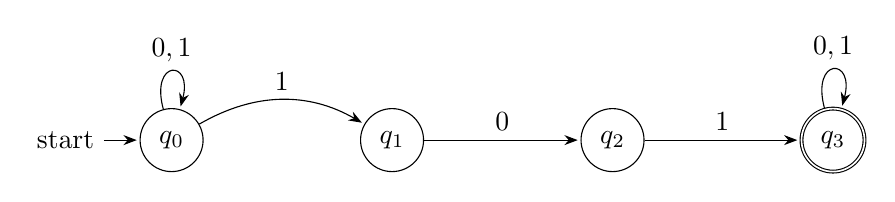
\begin{tikzpicture}[
->,
node distance=2.8cm,
every state/.style={minimum size=8mm}
]
\node[state,initial] (q0) {$q_0$};
\node[state,right of=q0] (q1) {$q_1$};
\node[state,right of=q1] (q2) {$q_2$};
\node[state,accepting,right of=q2] (q3) {$q_3$};

\path
(q0) edge[loop above] node{\(0,1\)} ()
(q0) edge[bend left] node[above]{\(1\)} (q1)
(q1) edge node[above]{\(0\)} (q2)
(q2) edge node[above]{\(1\)} (q3)
(q3) edge[loop above] node{\(0,1\)} ();
\end{tikzpicture}
\end{center}

\vspace{0.5em}

The branch \(q_0\to q_1\to q_2\to q_3\) verifies one guessed occurrence of \(101\).

\end{frame}

%------------------------------------------------
\begin{frame}{Why Is This Nondeterministic?}

At state \(q_0\), on input \(1\), the machine has two choices:

\[
\delta(q_0,1)=\{q_0,q_1\}.
\]

\vspace{1em}

Interpretation:

\begin{itemize}
\item stay in \(q_0\): ignore this \(1\);
\item move to \(q_1\): guess this \(1\) starts the pattern.
\end{itemize}

\vspace{1em}

Both possibilities are explored.

\end{frame}

%------------------------------------------------
\begin{frame}{Trace on Input \(0101\)}

Input:

\[
0101
\]

\vspace{1em}

At the final \(1\), there is a branch that has seen

\[
1 \rightarrow 10 \rightarrow 101.
\]

\vspace{1em}

So one branch reaches \(q_3\).

\[
q_3\in F
\]

Therefore, \(0101\) is accepted.

\end{frame}

%------------------------------------------------
\begin{frame}{Trace on Input \(1000\)}

Input:

\[
1000
\]

\vspace{1em}

The machine may guess the first \(1\) begins \(101\).

\pause

Then it reads \(0\), which is promising.

\pause

But the next symbol is \(0\), not \(1\).

\vspace{1em}

That branch dies.

\pause

No accepting branch exists.

Therefore, \(1000\) is rejected.

\end{frame}

%------------------------------------------------
\begin{frame}{Acceptance in an NFA}

Important rule:

\vspace{1em}

\begin{center}
\textbf{An NFA accepts if at least one computation path accepts.}
\end{center}

\vspace{1em}

Consequences:

\begin{itemize}
\item If one path accepts and many paths reject, the input is accepted.
\item If all paths reject or die, the input is rejected.
\end{itemize}

\end{frame}

%------------------------------------------------
\begin{frame}{Computation Tree View}

For an NFA, computation is a tree.

\begin{center}
\begin{tikzpicture}[
level distance=1.05cm,
sibling distance=2.8cm,
every node/.style={font=\small}
]
\node {\(q_0\)}
  child { node {\(q_0\)}
    child { node {\(q_0\)} }
    child { node {\(q_1\)} }
  }
  child { node {\(q_1\)}
    child { node {\(q_2\)} }
  };
\end{tikzpicture}
\end{center}

\vspace{0.5em}

If any leaf is accepting after the input is consumed, the NFA accepts.

\end{frame}

%------------------------------------------------
\begin{frame}[standout]
A DFA has one timeline.

An NFA has many possible timelines.
\end{frame}

%================================================
\section{Lecture 5C: Formal Definition of NFA}

%------------------------------------------------
\begin{frame}{Formal Definition}

A nondeterministic finite automaton is a 5-tuple

\[
M=(Q,\Sigma,\delta,q_0,F),
\]

where:

\begin{itemize}
\item \(Q\) is a finite set of states,
\item \(\Sigma\) is the input alphabet,
\item \(q_0\in Q\) is the start state,
\item \(F\subseteq Q\) is the set of accepting states,
\item \(\delta\) is the transition function.
\end{itemize}

\vspace{0.5em}

Only \(\delta\) differs from the DFA case.

\end{frame}

%------------------------------------------------
\begin{frame}{DFA versus NFA Transition Functions}

For a DFA:

\[
\delta:Q\times\Sigma\rightarrow Q.
\]

For an NFA:

\[
\delta:Q\times\Sigma\rightarrow \powset{Q}.
\]

\vspace{1em}

Here \(\powset{Q}\) means the set of all subsets of \(Q\).

\end{frame}

%------------------------------------------------
\begin{frame}{Why a Set of States?}

Suppose

\[
Q=\{q_0,q_1,q_2\}.
\]

Then

\[
\powset{Q}
=
\{
\emptyset,
\{q_0\},
\{q_1\},
\{q_2\},
\{q_0,q_1\},
\{q_0,q_2\},
\{q_1,q_2\},
\{q_0,q_1,q_2\}
\}.
\]

\vspace{0.5em}

An NFA transition may return any one of these subsets.

\end{frame}

%------------------------------------------------
\begin{frame}{Interpreting the Output of \(\delta\)}

\[
\delta(q,a)=\emptyset
\]

means no branch survives.

\vspace{1em}

\[
\delta(q,a)=\{r\}
\]

means exactly one next possibility.

\vspace{1em}

\[
\delta(q,a)=\{r,s,t\}
\]

means the computation branches into three possibilities.

\end{frame}

%------------------------------------------------
\begin{frame}{Formal Specification of the \(101\) NFA}

\[
Q=\{q_0,q_1,q_2,q_3\},
\qquad
\Sigma=\{0,1\},
\qquad
F=\{q_3\}.
\]

\[
q_0 \text{ is the start state.}
\]

\vspace{1em}

The transition function is:

\[
\begin{array}{c|cc}
\delta & 0 & 1\\
\hline
q_0 & \{q_0\} & \{q_0,q_1\}\\
q_1 & \{q_2\} & \emptyset\\
q_2 & \emptyset & \{q_3\}\\
q_3 & \{q_3\} & \{q_3\}
\end{array}
\]

\end{frame}

%------------------------------------------------
\begin{frame}{Notice the Difference}

In a DFA table, each entry is a state.

\[
q_0,\quad q_1,\quad q_2
\]

\vspace{1em}

In an NFA table, each entry is a set of states.

\[
\emptyset,\quad \{q_0\},\quad \{q_0,q_1\}
\]

\vspace{1em}

The table is just a precise way to define the transition function.

\end{frame}

%------------------------------------------------
\begin{frame}{Every DFA Is an NFA}

A DFA transition

\[
\delta(q,a)=r
\]

can be viewed as the NFA transition

\[
\delta(q,a)=\{r\}.
\]

\vspace{1em}

So every DFA is automatically an NFA.

\pause

\vspace{1em}

But is every NFA equivalent to some DFA?

That is the big question.

\end{frame}

%================================================
\section{Lecture 5D: More Examples}

%------------------------------------------------
\begin{frame}{Example: Strings Ending with \(01\)}

Let

\[
L=\{w\in\{0,1\}^*: w \text{ ends with }01\}.
\]

Examples:

\[
01,\quad 101,\quad 0001,\quad 1101.
\]

Non-examples:

\[
\eps,\quad 0,\quad 1,\quad 010,\quad 011.
\]

\end{frame}

%------------------------------------------------
\begin{frame}{NFA for Strings Ending with \(01\)}

\begin{center}
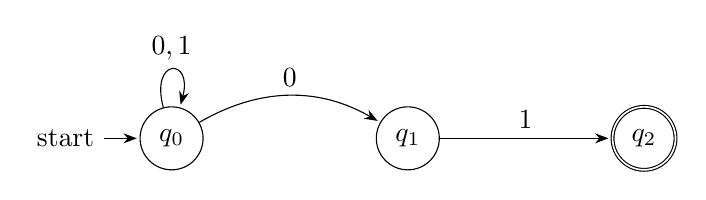
\begin{tikzpicture}[
->,
node distance=3cm,
every state/.style={minimum size=8mm}
]
\node[state,initial] (q0) {$q_0$};
\node[state,right of=q0] (q1) {$q_1$};
\node[state,accepting,right of=q1] (q2) {$q_2$};

\path
(q0) edge[loop above] node{\(0,1\)} ()
(q0) edge[bend left] node[above]{\(0\)} (q1)
(q1) edge node[above]{\(1\)} (q2);
\end{tikzpicture}
\end{center}

\vspace{0.5em}

The machine guesses which \(0\) is the second-last symbol.

\end{frame}

%------------------------------------------------
\begin{frame}{Why This Works}

For input

\[
110101
\]

the NFA may ignore early symbols.

\vspace{1em}

When it sees the final \(0\) before the last \(1\), it guesses:

\begin{center}
This \(0\) is the beginning of the suffix \(01\).
\end{center}

\vspace{1em}

If the next symbol is \(1\) and input ends, the machine accepts.

\end{frame}

%------------------------------------------------
\begin{frame}{Important Subtlety}

In the NFA for strings ending with \(01\), the accepting state has no outgoing transition.

\vspace{1em}

Why?

\pause

If the machine reaches the accepting state before the input ends, that branch dies on the next input symbol.

\vspace{1em}

Thus acceptance requires ending exactly at the accepting state.

\end{frame}

%------------------------------------------------
\begin{frame}{Example: Third Symbol from the End Is \(1\)}

Let

\[
L=\{w\in\{0,1\}^*: \text{the third symbol from the end of } w \text{ is }1\}.
\]

Examples:

\[
100,\quad 101,\quad 1101,\quad 00100.
\]

Non-examples:

\[
\eps,\quad 0,\quad 10,\quad 000,\quad 0100.
\]

\end{frame}

%------------------------------------------------
\begin{frame}{NFA Idea}

The machine scans the input.

Whenever it sees a \(1\), it may guess:

\begin{center}
This \(1\) is the third symbol from the end.
\end{center}

Then it must read exactly two more symbols and stop.

\end{frame}

%------------------------------------------------
\begin{frame}{NFA for Third Symbol from the End Is \(1\)}

\begin{center}
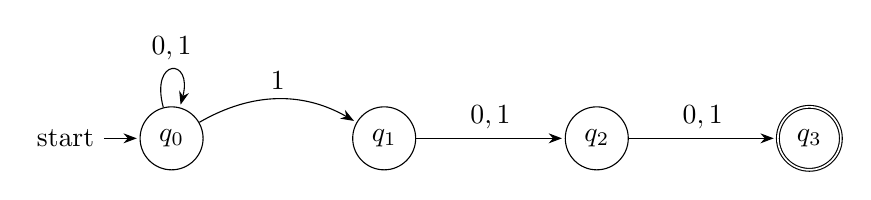
\begin{tikzpicture}[
->,
node distance=2.7cm,
every state/.style={minimum size=8mm}
]
\node[state,initial] (q0) {$q_0$};
\node[state,right of=q0] (q1) {$q_1$};
\node[state,right of=q1] (q2) {$q_2$};
\node[state,accepting,right of=q2] (q3) {$q_3$};

\path
(q0) edge[loop above] node{\(0,1\)} ()
(q0) edge[bend left] node[above]{\(1\)} (q1)
(q1) edge node[above]{\(0,1\)} (q2)
(q2) edge node[above]{\(0,1\)} (q3);
\end{tikzpicture}
\end{center}

\vspace{0.5em}

This NFA has only four states.

\pause

The equivalent DFA may need to remember the last three bits.

\end{frame}

%------------------------------------------------
\begin{frame}{Why NFAs Can Be Shorter}

NFAs can express:

\begin{center}
``There exists a good guess.''
\end{center}

\vspace{1em}

For the language

\[
\text{third symbol from the end is }1,
\]

the good guess is the position of that special \(1\).

\vspace{1em}

DFAs cannot guess; they must remember enough information deterministically.

\end{frame}

%------------------------------------------------
\begin{frame}{Example: At Least One \(0\) and At Least One \(1\)}

Let

\[
L=\{w\in\{0,1\}^*: w \text{ contains at least one }0
\text{ and at least one }1\}.
\]

\vspace{1em}

Examples:

\[
01,\quad 10,\quad 001,\quad 1110.
\]

Non-examples:

\[
\eps,\quad 000,\quad 111.
\]

\end{frame}

%------------------------------------------------
\begin{frame}{DFA Thinking for This Language}

A DFA may remember which symbols have appeared so far.

\[
\text{none},\quad
\text{only 0},\quad
\text{only 1},\quad
\text{both}.
\]

\vspace{1em}

This gives four natural states.

\pause

Here nondeterminism is not especially useful.

Not every language becomes simpler with NFAs.

\end{frame}

%------------------------------------------------
\begin{frame}{Example: Exactly the String \(101\)}

Let

\[
L=\{101\}.
\]

\vspace{1em}

This language contains exactly one string.

\pause

A machine for this language should accept \(101\), and reject everything else:

\[
\eps,\quad 1,\quad 10,\quad 1010,\quad 0101.
\]

\end{frame}

%------------------------------------------------
\begin{frame}{NFA for \(\{101\}\)}

\begin{center}
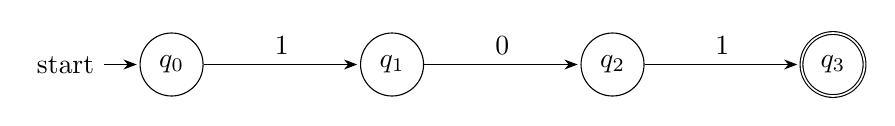
\begin{tikzpicture}[
->,
node distance=2.8cm,
every state/.style={minimum size=8mm}
]
\node[state,initial] (q0) {$q_0$};
\node[state,right of=q0] (q1) {$q_1$};
\node[state,right of=q1] (q2) {$q_2$};
\node[state,accepting,right of=q2] (q3) {$q_3$};

\path
(q0) edge node[above]{\(1\)} (q1)
(q1) edge node[above]{\(0\)} (q2)
(q2) edge node[above]{\(1\)} (q3);
\end{tikzpicture}
\end{center}

\vspace{0.5em}

No outgoing transitions are needed.

A missing transition means that branch dies.

\end{frame}

%================================================
\section{Lecture 5E: Special Languages and Empty Objects}

%------------------------------------------------
\begin{frame}{A Common Confusion}

Do not confuse:

\[
\emptyset
\]

and

\[
\{\eps\}.
\]

\vspace{1em}

They are very different languages.

\end{frame}

%------------------------------------------------
\begin{frame}{The Empty Language}

\[
\emptyset
\]

contains no strings.

\vspace{1em}

Not even the empty string.

\vspace{1em}

So:

\[
\eps\notin\emptyset.
\]

\end{frame}

%------------------------------------------------
\begin{frame}{NFA for the Empty Language}

\begin{center}
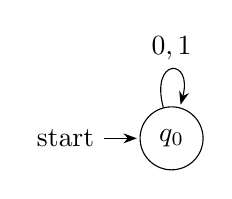
\begin{tikzpicture}[
->,
node distance=3cm,
every state/.style={minimum size=8mm}
]
\node[state,initial] (q0) {$q_0$};
\path
(q0) edge[loop above] node{\(0,1\)} ();
\end{tikzpicture}
\end{center}

\vspace{1em}

There are no accepting states:

\[
F=\emptyset.
\]

Therefore, no input is accepted.

\end{frame}

%------------------------------------------------
\begin{frame}{The Language Containing Only the Empty String}

\[
\{\eps\}
\]

contains exactly one string: the empty string.

\vspace{1em}

So:

\[
\eps\in\{\eps\}.
\]

But:

\[
0\notin\{\eps\},\qquad 1\notin\{\eps\}.
\]

\end{frame}

%------------------------------------------------
\begin{frame}{NFA for \(\{\eps\}\)}

\begin{center}
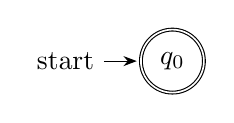
\begin{tikzpicture}[
->,
node distance=3cm,
every state/.style={minimum size=8mm}
]
\node[state,initial,accepting] (q0) {$q_0$};
\end{tikzpicture}
\end{center}

\vspace{1em}

The start state is accepting.

\vspace{0.5em}

But there are no transitions on \(0\) or \(1\), so any nonempty input is rejected.

\end{frame}

%------------------------------------------------
\begin{frame}{Compare Carefully}

\[
\emptyset
\]

has zero strings.

\vspace{1em}

\[
\{\eps\}
\]

has one string.

\vspace{1em}

\pause

Therefore:

\[
\emptyset\neq \{\eps\}.
\]

\end{frame}

%------------------------------------------------
\begin{frame}{More Special Languages}

Over alphabet \(\Sigma=\{0,1\}\):

\[
\Sigma^*
\]

all binary strings.

\vspace{0.5em}

\[
\Sigma^+
\]

all nonempty binary strings.

\vspace{0.5em}

\[
\emptyset
\]

no strings.

\vspace{0.5em}

\[
\{\eps\}
\]

only the empty string.

\end{frame}

%------------------------------------------------
\begin{frame}{NFA for \(\Sigma^*\)}

\begin{center}
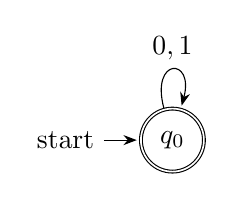
\begin{tikzpicture}[
->,
node distance=3cm,
every state/.style={minimum size=8mm}
]
\node[state,initial,accepting] (q0) {$q_0$};
\path
(q0) edge[loop above] node{\(0,1\)} ();
\end{tikzpicture}
\end{center}

\vspace{1em}

Every string is accepted, including \(\eps\).

\end{frame}

%------------------------------------------------
\begin{frame}{NFA for \(\Sigma^+\)}

\begin{center}
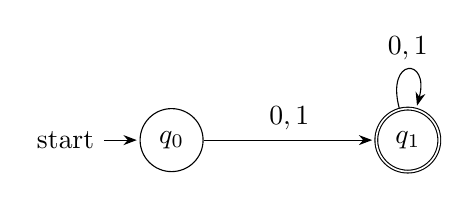
\begin{tikzpicture}[
->,
node distance=3cm,
every state/.style={minimum size=8mm}
]
\node[state,initial] (q0) {$q_0$};
\node[state,accepting,right of=q0] (q1) {$q_1$};

\path
(q0) edge node[above]{\(0,1\)} (q1)
(q1) edge[loop above] node{\(0,1\)} ();
\end{tikzpicture}
\end{center}

\vspace{1em}

All nonempty strings are accepted.

The empty string is rejected.

\end{frame}

%------------------------------------------------
\begin{frame}{Finite Languages Are Regular}

Every finite language can be recognized by a finite automaton.

\vspace{1em}

Example:

\[
L=\{00,11,101\}.
\]

\vspace{1em}

We can build one path for each string.

\pause

Nondeterminism makes this construction very natural.

\end{frame}

%------------------------------------------------
\begin{frame}{NFA for a Finite Language}

For

\[
L=\{00,11,101\},
\]

create a new start state and branch into three paths:

\[
00,\qquad 11,\qquad 101.
\]

\vspace{1em}

This idea will later become useful for regular expressions and closure properties.

\end{frame}

%================================================
\section{Lecture 5F: Epsilon Transitions}

%------------------------------------------------
\begin{frame}{Can the Machine Move Without Reading Input?}

An NFA may contain transitions labeled

\[
\eps.
\]

\vspace{1em}

These consume no input symbol.

\vspace{1em}

They are called \textbf{\(\eps\)-transitions}.

\end{frame}

%------------------------------------------------
\begin{frame}{How to Think About \(\eps\)-Transitions}

An \(\eps\)-transition means:

\begin{center}
The machine changes state without reading input.
\end{center}

\vspace{1em}

Possible interpretations:

\begin{itemize}
\item changing its mind,
\item jumping to a submachine,
\item making a free nondeterministic choice,
\item starting a different module.
\end{itemize}

\end{frame}

%------------------------------------------------
\begin{frame}{Example: Accepting \(\{a,b\}\)}

\begin{center}
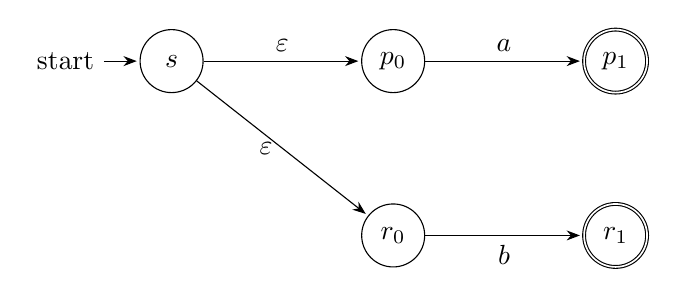
\begin{tikzpicture}[
->,
node distance=2.4cm,
every state/.style={minimum size=8mm}
]
\node[state,initial] (s) {$s$};
\node[state,right=2cm of s] (a0) {$p_0$};
\node[state,accepting,right=2cm of a0] (a1) {$p_1$};
\node[state,below=1.4cm of a0] (b0) {$r_0$};
\node[state,accepting,right=2cm of b0] (b1) {$r_1$};

\path
(s) edge node[above]{\(\eps\)} (a0)
(s) edge node[left]{\(\eps\)} (b0)
(a0) edge node[above]{\(a\)} (a1)
(b0) edge node[below]{\(b\)} (b1);
\end{tikzpicture}
\end{center}

\vspace{0.5em}

The machine freely chooses the \(a\)-path or the \(b\)-path.

\end{frame}

%------------------------------------------------
\begin{frame}{Why \(\eps\)-Transitions Are Useful}

They make automata modular.

\vspace{1em}

If we already have machines for \(L_1\) and \(L_2\), \(\eps\)-transitions let us combine them easily.

\vspace{1em}

This will later help us prove closure under:

\begin{itemize}
\item union,
\item concatenation,
\item star.
\end{itemize}

\end{frame}

%------------------------------------------------
\begin{frame}{Union Idea}

To recognize

\[
L_1\cup L_2,
\]

make a new start state.

\vspace{1em}

Use \(\eps\)-transitions to enter either machine:

\[
\text{new start}
\overset{\eps}{\longrightarrow}
M_1
\qquad
\text{or}
\qquad
\text{new start}
\overset{\eps}{\longrightarrow}
M_2.
\]

\vspace{1em}

Accept if either submachine accepts.

\end{frame}

%------------------------------------------------
\begin{frame}{Concatenation Idea}

To recognize

\[
L_1L_2,
\]

run the machine for \(L_1\), then jump to the machine for \(L_2\).

\vspace{1em}

Use \(\eps\)-transitions from accepting states of \(M_1\) to the start state of \(M_2\).

\vspace{1em}

The NFA guesses where the first part ends and the second part begins.

\end{frame}

%------------------------------------------------
\begin{frame}{Star Idea}

To recognize

\[
L^*,
\]

we must allow:

\[
0,\;1,\;2,\;3,\ldots
\]

copies of strings from \(L\).

\vspace{1em}

\(\eps\)-transitions allow us to loop back and repeat the machine.

\vspace{1em}

This is one reason NFAs are so convenient.

\end{frame}

%================================================
\section{Lecture 5G: Nondeterminism in the Larger Story}

%------------------------------------------------
\begin{frame}{Nondeterminism and Regular Languages}

NFAs do not change which languages are regular.

\vspace{1em}

But they often make descriptions simpler.

\vspace{1em}

They are useful because they separate two questions:

\begin{itemize}
\item How naturally can we describe a language?
\item How powerful is the model?
\end{itemize}

\end{frame}

%------------------------------------------------
\begin{frame}{Nondeterminism Beyond Automata}

The same idea reappears in later topics:

\begin{itemize}
\item nondeterministic Turing machines,
\item the class NP,
\item SAT and NP-completeness,
\item search problems,
\item proof verification,
\item optimization,
\item automated reasoning.
\end{itemize}

\vspace{1em}

This is why NFA is more than a technical definition.

\end{frame}

%------------------------------------------------
\begin{frame}{A Preview of NP}

Later in complexity theory, you will see:

\[
\text{NP}
\]

as the class of problems where a proposed solution can be verified efficiently.

\vspace{1em}

Nondeterminism gives one mathematical way to model guessing such a solution.

\vspace{1em}

NFA is our first small encounter with that idea.

\end{frame}

%------------------------------------------------
\begin{frame}{Think Before Next Lecture}

We now have two models:

\[
\text{DFA}
\qquad
\text{and}
\qquad
\text{NFA}.
\]

\vspace{1em}

NFAs seem more flexible.

They can branch.

They can guess.

They can use \(\eps\)-transitions.

\vspace{1em}

Question:

\begin{center}
Do they recognize more languages?
\end{center}

\end{frame}

%------------------------------------------------
\begin{frame}[standout]
A nondeterministic machine seems more powerful.

Next lecture:

\[
\text{Every NFA can be simulated by a DFA.}
\]
\end{frame}

%================================================
\section{Practice Problems}

%------------------------------------------------
\begin{frame}{Practice: Predict the Language}

For each NFA, determine the language.

\vspace{1em}

\begin{enumerate}
\item A single accepting start state with no transitions.
\item A single non-accepting start state with loops on \(0,1\).
\item A path labeled \(0,1,0\) ending in an accepting state.
\item A start state with \(\eps\)-branches to paths \(00\), \(11\), and \(101\).
\end{enumerate}

\end{frame}

%------------------------------------------------
\begin{frame}{Practice: Design NFAs}

Design NFAs for:

\begin{enumerate}
\item strings ending with \(101\);
\item strings containing \(000\);
\item strings whose fourth symbol from the end is \(1\);
\item \(\{0,11,101\}\);
\item all nonempty strings over \(\{a,b\}\).
\end{enumerate}

\end{frame}

%------------------------------------------------
\begin{frame}{Key Takeaways}

\begin{itemize}
\item A DFA has exactly one next state.
\item An NFA may have many possible next states.
\item A branch may die.
\item An input is accepted if at least one branch accepts.
\item \(\eps\)-transitions consume no input.
\item NFAs often make language descriptions simpler.
\item Nondeterminism is a central abstraction in TCS.
\end{itemize}

\end{frame}

%------------------------------------------------
\begin{frame}[standout]
Nondeterminism is the mathematics of possibility.

Next:

possibility can still be simulated deterministically.
\end{frame}

%================================================
\end{document}
